\section{Versuch}
\subsection{Versuchsaufbau}
Der Aufbau des HeNe-Lasers ist in Abbildung \ref{fig:hene2} zu sehen.

\begin{figure}
	\centering
	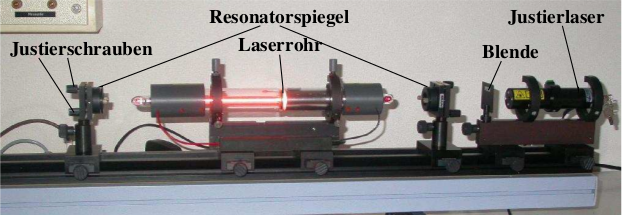
\includegraphics[width=0.5\textwidth]{hene2.png}
	\caption{Aufbau des HeNe-Lasers}
	\label{fig:hene2}
\end{figure}

\noindent Es steht eine optische Schiene zur Verfügung, auf der ein Justierlaser mit Wellenlänge \(\lambda=532\)nm angebracht ist. Hinter dem Justierlaser und am Ende der optischen Schiene ist ein Schirm mit Fadenkreuz befestigt. Des Weiteren ist ein Schirm für die Betrachtung der Interferenzmuster Teil des Aufbaus.

\noindent Es gibt ein Laserrohr und mehrere Resonatorspiegel, die den Laserresonator bilden. Für die Messung der Moden steht ein Wolfram Draht zur Verfügung. Die Polarisation wird mit einem Polarisationsfilter gemessen. Die Wellenlänge mit einem Gitter.

\noindent Die Intensität des Lasers wird durch einen Strom nach Auftreffen einer Photodiode aufgenommen. Außerdem gibt es eine Spannungsquelle zur Anregung des Heilums und der Aktivierung des Lasers.

\subsection{Versuchsdurchführung}
Zunächst wird der HeNe-Laser justiert. Dazu wird sich des Justierlasers bedient, welcher schon voreingestellt ist. Es wird ein Resonatorspiegel auf die optische Schiene gestellt und so ausgerichtet, dass der reflektierte Strahl des Justierlasers wieder in der Mitte des Fadenkreuzes liegt. Dies wird mit dem nächsten Spiegel wiederholt. Dann wird das Laserrohr angebracht. Auch hier wird wieder der Strahl des Justierlasers auf die Mitte des Fadenkreuzes eingestellt. Danach wird der Justierlaser ausgeschaltet und die Spannungsquelle eingeschaltet.

\noindent Damit die Lasertätigkeit einsetzt, werden noch die Schrauben der drei Komponenten feinjustiert. Ist alles richtig eingestellt, erscheint ein roter Lichtstrahl zwischen den Brewster-Fenstern des Laserrohrs und den Resonatorspiegeln.

\noindent Zur Überprüfung der Stabilitätsbedingung wird der Strahl des HeNe-Lasers auf eine Photodiode konzentriert. Dann wird nach und nach der Abstand der Spiegel zum Laserrohr vergrößert, also die Länge des Resonators erhöht, und der durch die Diode gemessene Strom aufgenommen. Dies wird für zwei verschiedene Spiegel-Konstellationen durchgeführt.

\noindent Weiterführend werden zwei verschiedene TEM Moden gemessen. Einmal die \(\text{TEM}_{00}\) Grundmode und die \(\text{TEM}_{10}\) Mode. Erste wird durch Aufnahme des Stromes durch die Photodiode gemessen, wobei eine Linse hinter zwischen Resonatorspiegel und Photodiode befestigt wird. Für die \(\text{TEM}_{10}\) Mode wird noch ein Wolfram-Draht auf der optischen Schiene befestigt.

\noindent Die Polarisation wird wieder durch Aufnahme der Intensität des Laserstrahls durch die Photodiode gemessen, jedoch bei davor befestigtem Polarisationsfilter. Es werden Werte für die Winkel 0°-360° aufgenommen.

\noindent Zuletzt wird ein Gitter hinter den Resonatorspiegel gestellt und statt der Photodiode ein Schirm verwendet, um die Abstände der Intensitätsmaxima mit einem Maßband zu messen. Das Hauptmaxima wird ermittelt, indem das Gitter gedreht wird und somit die ''Gitterkonstante'' verändert wird, die Maxima also einen kleineren bzw. größeren Abstand haben, das Hauptmaximum allerdings vom Ort her unverändert bleibt.